\section{Overview} \label{sec:overview}

This section first introduces \xxx's architecture with its key components, and 
then discusses which types of anlyses are suitable to run in \xxx. We mainly 
consider server applications (\eg, \apache and \clamav) because they provide 
online service and thus require significant analyses to guarantee software 
quality. Utility programs can also be easily run in our \xxx.

\subsection{\xxx Architecture} \label{sec:arch}

\xxx's deployment is similar to a typical \smr's. In a \xxx-replicated
system, a set of 2\v{f}+1 machines (nodes) are set up within a LAN,
and each node runs an instance of \xxx containing the same server
program running with or without an anlysis tool. Once the \xxx system starts, 
one node becomes the \emph{primary} node which proposes the order of requests 
to execute, and the others become backup nodes which follow the primary's 
proposals. Up to \v{f} nodes run an heavyweight anlysis tool on each, so at 
least \v{f}+1 nodes run the native application or lightweight analyses so that 
they can reach consensus on inputs and process requests fast. An arbitrary 
number of clients in LAN or WAN send network requests to the primary and get 
responses. 


\begin{figure}[t]
\vspace{.20in}
\centering
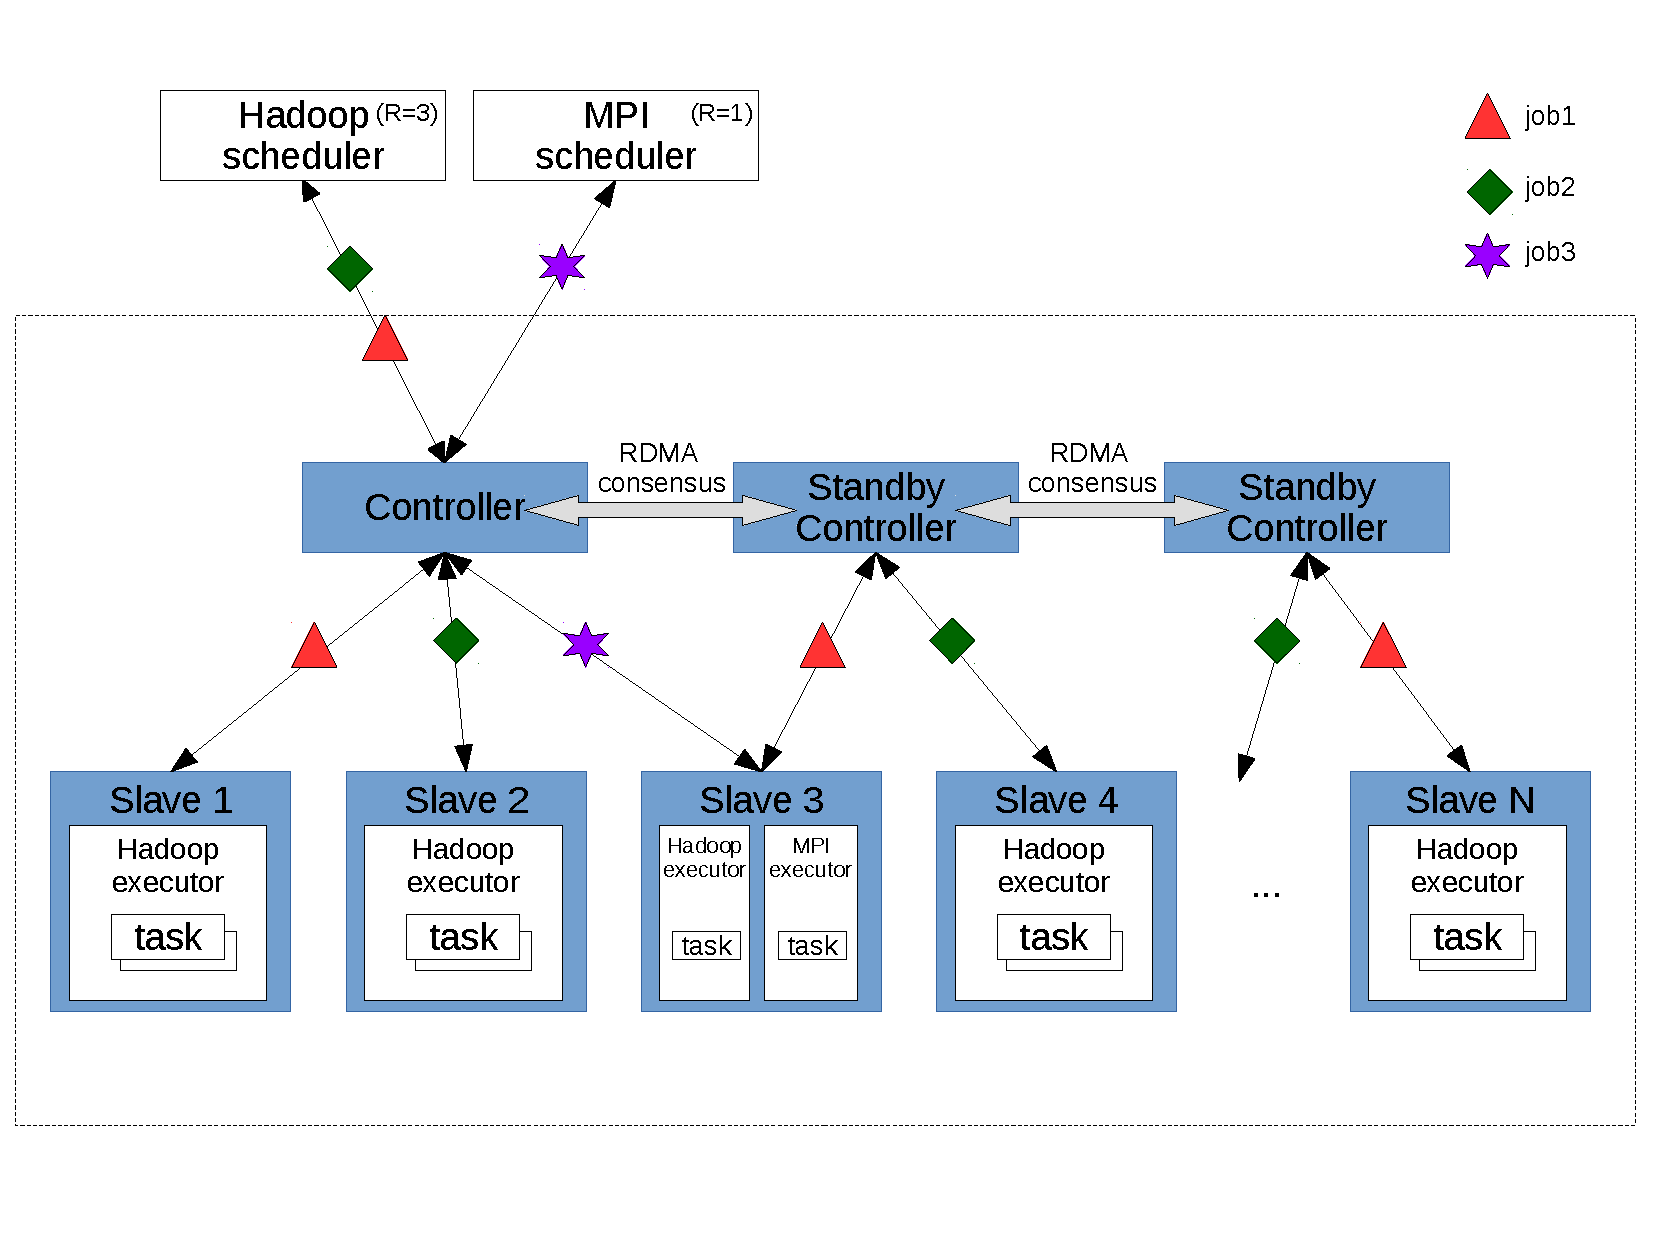
\includegraphics[width=.5\textwidth]{figures/arch}
\vspace{-.20in}
\caption{{\em The \xxx Architecture.} \xxx components are shaded (and in
  green).} \label{fig:arch}
\vspace{-.05in}
\end{figure}

Figure~\ref{fig:arch} shows an instance of \xxx running on 
each node. The abstraction contains three main components, the \paxos consensus 
component, the \dmt scheduler, the checkpointer component. A server program 
runs transparently in a \xxx instance with or without an analysis. Neither the 
server or the analysis is aware of of \xxx's components.

To support general server programs, \xxx chooses the POSIX socket API as
consensus interface. \xxx enforces two kinds of orders for socket
operations.  For requests coming from the clients, such as \connect and
\send requests, \xxx enforces that all nodes see the same totally ordered
sequence of these requests using the \paxos and socket API interposition
components.  (\xxx does not need to order the blocking socket operations
in the clients because we mainly focus on analyses for server applications.)


The \paxos consensus component is a \xxx instance's gateway.  It accepts socket
requests from the clients and invoke a \paxos consensus instance on this 
operation. Once a consensus is reached. This component is also the only \xxx 
component that communicates among different \xxx instances. For practicality, 
\xxx uses a well-known \paxos engineering approach~\cite{paxos:practical} in 
which only the primary invokes consensus request during normal operations.

The \dmt component runs within the same process as a server replica, and
enforces the same logical clocks for inter-thread communication
operations. \xxx leverages the \parrot~\cite{parrot:sosp13} \dmt runtime
system because it was shown to run fast on a wide range of 108 popular
multithreaded programs. We choose this \dmt runtime because it is fast (\ie, 
12.7\% overhead for a wide range of 108 popular multithreaded programs) and 
transparent to the application.

Specifically, \parrot uses a runtime technique called \ldpreload to dynamically 
intercept \pthread synchronizations (\eg, \mutexlock) issued by an executable 
and enforces a well-define, round-robin schedule on these synchronization 
operations for all threads, practically eliminating nondeterminism in thread
synchronizations. Although \parrot is not designed to resolve data races
deterministically, \xxx's replication tolerates data races that have
fail-stop consequences (see \S\ref{sec:limit}), and can further catch the
other data races by running a race detector on a backup node (see
\S\ref{sec:discussion}).  \xxx augments the \dmt component to schedule the
return points of socket operations in server replicas, too, to ensure that
requests are admitted exactly at the same logical time across replicas.

The checkpointer component is invoked every minute in a non-primary node that 
is running the native application and nodes that are running an analysis. Each 
checkpoint is associated with the index of the last executed socket operation, 
so that \xxx can consistently match up with the execution states of native 
executions and various analysis executions. To perform checkpoints 
transparently without affecting application's executions and analyses, \xxx 
leverages \criu, a popular, open source process checkpoint tool that supports 
CPU registers, memory, etc. Each checkpoint operation is only performed on the 
server program and the \dmt schculer; the \paxos consensus component does not 
require checkpoints because we explicitly design it to be stateless (all socket 
operations have been persisitently logged).

% Our model. Multiple writer multiple reader.

\subsection{Discussion} \label{sec:discuss}

Many analyses can be done asynchronously.

For instance, race detection. A previous detector sacrifice soundness (may miss 
bugs) for better performance. With our framework, this analysis can regain 
soundness, while the application can still run fast.

Extra guarantees. Some nodes fail. Role change.